\subsubsection{\theoryC{Relaxion at the HL-LHC}}
\contributors{E. Fuchs, M. Schlaffer}\rt{There are comments to address.}
%{\bf Author(s): ?}

%\paragraph*{The relaxion framework}
The relaxion mechanism~\cite{Graham:2015cka} addresses the hierarchy problem 
differently than conventional symmetry-based solutions. 
In this framework, the Higgs mass is stabilized dynamically by the relaxion, a pseudo-Nambu-Goldstone boson.
The Higgs mass is scanned by the evolution of the relaxion field. Eventually, the relaxion stops at the field value
where the Higgs mass is much smaller than the theory's cutoff, hence addressing the fine tuning problem.  
Relaxion models do not require top, gauge or Higgs partners at the TeV scale. The possible mass range for the relaxion ranges from sub-eV to tens of GeV.  Hence this framework can lead to signatures relevant for cosmology, for the low-energy precision frontier, for the intensity frontier, and for the high energy collider frontier. For detailed studies see \citerefs{Flacke:2016szy,Choi:2016luu,Frugiuele:2018coc}.

The aspects of the relaxion mechanism that are relevant for the phenomenology at colliders are summarized in the following.
The effective scalar potential of
the theory depends both on the Higgs doublet $H$ and the relaxion $\phi$,
\begin{align}
  V(H,\phi)&=\mu^2(\phi) H^\dagger H+\lambda (H^ \dagger H)^2 + V_{\rm sr}(\phi)+ V_\text{br}(h,\phi)\, ,\label{eq:pot}\\
  \mu^2(\phi)&=-\Lambda^2+g \Lambda \phi + \dots   \, ,
\label{eq:mu2}
\end{align}
where $\Lambda$ is the cutoff scale of a Higgs loop.
The relaxion scans $\mu^2$ via the slow-roll potential
\begin{equation}
  V_{\rm sr}(\phi)=r g\Lambda^3 \phi\,,
\label{eq:roll}
\end{equation}
where $g$ is a small dimension-less coupling and $r > 1/ (16 \pi^2)$ due to naturalness
requirements. Once $\mu^2(\phi)$ becomes negative, the Higgs gets a \vev
$v^2(\phi)=-\frac{\mu^2(\phi)}{\lambda}$. The non-zero \vev activates a periodic (model-dependent)
backreaction potential $V_\text{br}$ associated with the backreaction scale $\Lambda_{\textrm{br} }$ that eventually
stops the rolling of the relaxion at a value $\phi_0$, where $v(\phi_0)=246\,\textrm{GeV}$.  Generically, the
relaxion mechanism leads to \cp violation and as a result, the relaxion $\phi$ mixes with the
Higgs $h$ and inherits its couplings to SM fields~\cite{Flacke:2016szy,Choi:2016luu}.  The relaxion
mass $m_{\phi}$ and the mixing angle $\sin\theta$ can be expressed as
\begin{align}
m_{\phi} &\simeq \frac{ \Lambda_{\textrm{br} }^2}{f} \sqrt{c_0 }\,,
\label{eq:mphiApprox}\\
\sin{\theta}
 &\simeq 8   \frac{\Lambda_{\textrm{br} }^4}{v^3 f} s_0 \,,
\label{eq:sinth}
\end{align}
where $s_0\equiv \sin\phi_0, ~c_0\equiv \cos\phi_0$, and $f$ is the scale where the shift symmetry of the backreaction potential
is broken. Combining \eqs{eq:mphiApprox} and~\eqref{eq:sinth} with
$4 \Lambda_{\textrm{br} }^2 s_0 < v^2\sqrt{c_0}$, which is fulfilled due to the suppressed value of $s_0$ at the endpoint of
the rolling~\cite{Choi:2016luu}, the mixing angle as a function of the relaxion mass is
approximately bounded by
\begin{equation}
 \sin\theta \leq 2\frac{m_{\phi}}{v}\,.
 \label{eq:maxmixNatural}
\end{equation}
This upper bound on the relaxion-Higgs mixing is indicated by the black line in \fig{fig:DirIndirHLLHC}.

  \begin{figure}[t!]
 \begin{center}
  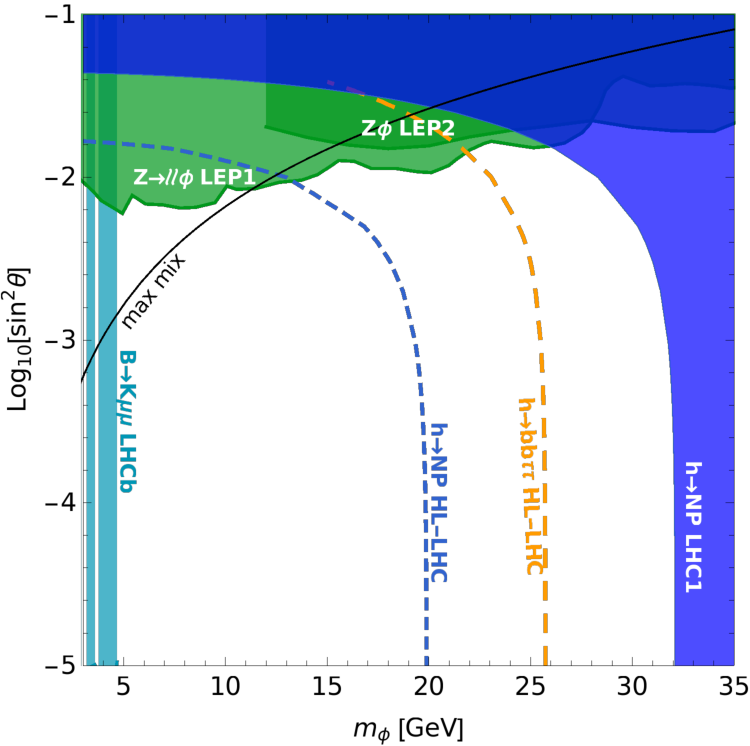
\includegraphics[height=0.5\textwidth]{\main/section7OtherSignatures/img/DirIndirLHC.pdf}
    \caption{ Bounds and projections for processes at hadron and
    lepton colliders.  $Z\to Z^*\phi\to \ell\bar \ell \phi$ at LEP1 with
    $\sqrt{s}=M_Z$~\cite{Acciarri:1996um} and $e^+e^-\to Z\phi$ at LEP2 with
    $\sqrt{s}=192$--$202\,\textrm{GeV}$~\cite{Schael:2006cr}. 
    Bound from $B^+\to K^+ \mu^+ \mu^-$ at LHCb~\cite{Aaij:2012vr,Aaij:2015tna}. 
    Direct searches for exotic Higgs decays at the HL-LHC in
    the $bb\tau\tau$ channel inferred from \citeref{CMS:2018lqr} (orange, dashed).
    Upper bound on $\textrm{BR}(h\to\textrm{NP})$ from Higgs coupling fits at the LHC Run-1 (blue area, 95\%~\cl) and projection for the HL-LHC with $3\,\textrm{ab} ^{-1}$ (blue, dashed, 68\%~\cl). 
    The maximal mixing
    according to \eq{eq:maxmixNatural} is indicated by the black line.  }
  \label{fig:DirIndirHLLHC}
 \end{center}
\end{figure} 

Moreover, in the broken phase a trilinear relaxion-relaxion-Higgs coupling $c_{\phi\phi h}$ is
generated~\cite{Flacke:2016szy,Frugiuele:2018coc},
\begin{align}
 c_{\phi\phi h} &= \frac{\Lambda_{\textrm{br} }^4}{v f^2} c_0 c_{\theta}^3
 - \frac{2 \Lambda_{\textrm{br} }^4  }{v^2 f} s_0 c_{\theta}^2 s_{\theta}
- \frac{\Lambda_{\textrm{br} }^4}{2f^3} s_0 c_{\theta}^2 s_{\theta}
- \frac{2\Lambda_{\textrm{br} }^4}{v f^2} c_0 c_{\theta} s_{\theta}^2
+ 3v \lambda c_{\theta} s_{\theta}^2
                  + \frac{\Lambda_{\textrm{br} }^4 }{v^2 f} s_0 s_{\theta}^3\,,
                  \label{eq:phiphih}
\end{align}
where $s_\theta\equiv \sin\theta,~c_\theta\equiv \cos\theta$.
Thus a bound on $c_{\phi\phi h}$ constrains the $(m_\phi,\sin\theta)$ parameter space.
In the limit of small mixing, \eq{eq:phiphih} reduces to
$ c_{\phi\phi h}  \simeq m_{\phi}^2/v$\,,
therefore directly constraining the mass. 

%\paragraph*{Exotic Higgs decay $\boldsymbol{h\to\phi\phi}$} 
There are two complementary ways to constrain $c_{\phi\phi h}$ via the exotic Higgs decay $h\to\phi\phi$: searching directly for the decay products of the $\phi$ pair, or bounding this branching ratio by a global fit of Higgs couplings.
 
%\paragraph*{General bound on $\textrm{BR}(\boldmath{h}\to \textrm{NP})$ } 
Concerning the Higgs phenomenology, the relaxion can be viewed as a singlet extension of the SM with a mixing of $\phi$ and $h$. The Higgs couplings to SM particles are reduced by the universal coupling modifier $\kappa\equiv \cos\theta$ and the total Higgs width 
$\Gamma_h^{\rm tot} = \cos^2\theta\, \Gamma_h^{\rm tot,SM} + \Gamma_h^{\rm NP}$
contains the NP contribution $\Gamma_h^{\rm NP} = \Gamma(h\to\phi\phi)$.
For the LHC, $\textrm{BR}(h\to\textrm{NP})$ has been constrained via a Higgs coupling fit to Run-1 data to be at most $20\%$ at the 95\%~\cl and the projected limit of $4.3\%$ at the 68\%~\cl has been worked out for the HL-LHC in \citeref{Bechtle:2014ewa}.\rt{Agree with and possibly refer to WG2 on this.} The resulting bounds in the $(m_\phi, \sin\theta)$ plane are shown in \fig{fig:DirIndirHLLHC}.

\begin{figure}[t!]
 \begin{center}
  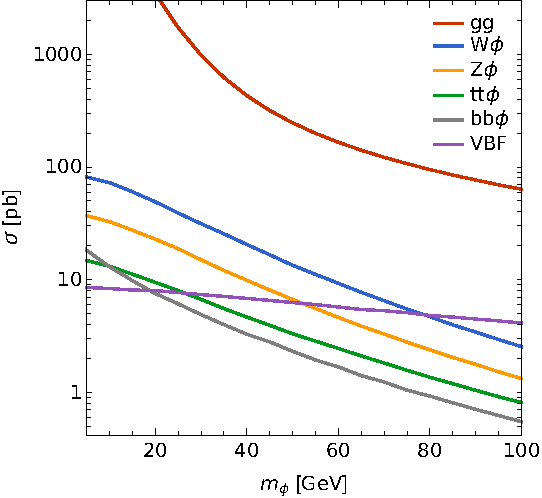
\includegraphics[width=0.49\textwidth]{\main/section7OtherSignatures/img/prod_xsec_had}\hfill
  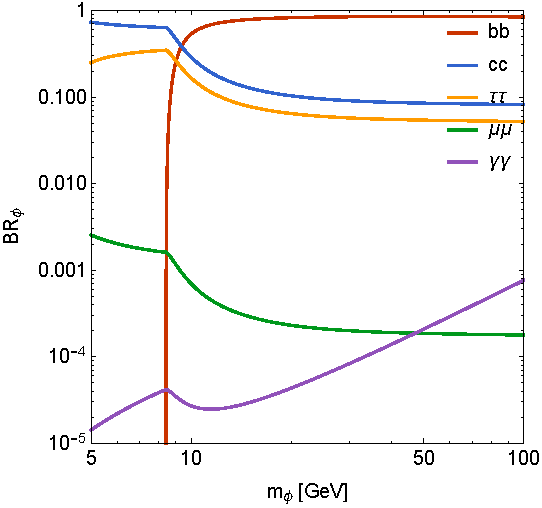
\includegraphics[width=0.49\textwidth]{\main/section7OtherSignatures/img/PlotBR}
  \caption{Production and decay of $\phi$ for $\sin^2\theta=1$.
    \textbf{Left:} Hadronic cross sections, $\sigma(pp\to X)$ at $\sqrt{s}=13\,\textrm{TeV}$
    for $X=\phi$ (via gluon fusion), $W\phi$, $Z\phi$, $t\bar t\phi$, $b\bar b\phi$, and $\phi jj$
    (via VBF).  The $\sigma(pp\to\phi)$ via gluon fusion is calculated using \texttt{ggHiggs
      v3.5}~\cite{Ball:2013bra,Bonvini:2014jma,Bonvini:2016frm,Ahmed:2016otz} at N$^3$LO including
    N$^3$LL resummation without a $p_T$-cut.  The remaining hadronic cross sections are obtained
    from \MGvATNLO \cite{Alwall:2014hca} at NLO with $p_T(\phi)>20\,\textrm{GeV}$.
    \textbf{Right:} Branching ratios
    ${\rm BR}(\phi\to b\bar b,\, c\bar c,\, \tau^+\tau^-, \mu^+\mu^-, \gamma\gamma)$.
   }
   \label{fig:prod_decay}
 \end{center}
\end{figure}

The parameter space probed by the HL-LHC enters the region below the upper
 bound of the mixing and is therefore relevant for the model. The HL-LHC may exclude a
 relaxion mass above $20\,\textrm{GeV}$ for vanishing $\sin\theta$.
 In comparison, direct relaxion production via $B\to K\phi$,
 $\phi\to\mu\mu$ at LHCb excludes $2m_\mu \leq m_\phi \lesssim 5\,\textrm{GeV}$ also for $\sin\theta$ smaller
 than shown in \fig{fig:DirIndirHLLHC}. In contrast, the bounds set by LEP1 via
 the 3-body $Z$-decay into $f\bar f\phi$ and by LEP2 via relaxion strahlung in $Z\phi$ production
 are sensitive only to mixing angles of order  $\sin^2\theta \gtrsim 10^{-2}$ and therefore constrain mostly
 parameter space above the theoretically motivated maximal mixing.
Furthermore, the stronger bound reachable at the HL-LHC, compared to the Run-1 one, is highly beneficial for constraining the relaxion mass space down to small mixing angles.
 
% \paragraph*{Searches for the relaxion decay products}
Each relaxion from the Higgs decay further decays into a pair of SM particles, resulting in a four-particle final state $F$. The ATLAS and CMS
searches for such signatures yield $m_{\phi}$-dependent bounds on
$(\sigma_h/\sigma_h^{\rm SM}) \times {\rm BR}\left(h\to\phi\phi \to F\right)$.
However, none of the current
searches~\cite{CMS:2018lqr,Khachatryan:2017mnf,Aaboud:2018esj,CMS:2018wii,CMS-PAS-HIG-16-035,Aaboud:2018fvk,Aaboud:2018iil,Aaboud:2018gmx} is sensitive enough to probe parts of the relaxion parameter space displayed in
\fig{fig:DirIndirHLLHC}, \textit{i.e.}\rt{Notation for i.e.}~$5\,\textrm{GeV} \leq m_{\phi} \leq 35\,\textrm{GeV}$
and $10^{-5}\leq \sin^2\theta \leq 10^{-1}$. 
In contrast, the HL-LHC can probe parts of the relevant parameter space via these channels.
We estimate the potential reach of the
HL-LHC with 3 ab$^{-1}$ by rescaling the current limits by the ratio of luminosities and, in the case
of Run-1 limits at $\sqrt{s}=8\,\textrm{TeV}$, additionally by the ratio of Higgs production cross sections at
$8$ and $13\,\textrm{TeV}$ in the dominant channels~\cite{xsecratio}.
According to this scaling, we find that the strongest bound at the HL-LHC is expected in the $bb\tau\tau$ channel, excluding $m_{\phi}>26\,\textrm{GeV}$ as shown in \fig{fig:DirIndirHLLHC}. \rt{In \fig{fig:DirIndirHLLHC} the same bound on $h\to NP$ is shown at 95\%~\cl from Run-1 and at 68\%~\cl for HL-LHC.}

% \paragraph*{Production modes in proton collisions}

Concerning the relaxion direct production at colliders,\rt{There is no result beyond plotting the cross sections at LHC for the direct production of relaxions. Maybe we can remove this part.} similarly to the Higgs, the dominant production modes for the relaxion are gluon fusion ($ p  p \to \phi $), relaxion strahlung ($ p  p \to Z \phi,~W\phi$),  $\left\lbrace t\bar t,~b\bar b \right\rbrace$-associated production, and vector boson fusion (VBF, $p p \to \phi j j$).
The cross sections of these processes are shown for $\sin\theta=1$ in the left panel of \fig{fig:prod_decay}. 
%
For the HL-LHC, a promising channel is relaxion strahlung due to the relatively large cross sections in combination with the presence of a massive gauge boson that can be tagged. Various decay modes can be considered, see the right panel of \fig{fig:prod_decay}.
So far the $Z\phi$ and $W\phi$ searches do not cover the challenging low-mass range. With high luminosity, extending these searches to lower masses could yield complementary bounds.


